\chapter{Model Validation}\label{ch:modValPerf}
\section{Static Modelling}
\todo[color=06modelValidationAndPerformance]{Model Validation and Performance}
To validate the model acquired in Chapter \ref{ch:mathmodel}, we ran a second test with the 
same setup as described in Chapter \ref{ch:experiment}. Coefficients were determined for pump models,
for every percentage of the valve opening.

Equation \ref{eq:pumpHeadModel60} and \ref{eq:pumpPowerModel60} represent the modeled Flow and Power 
Consumption for 60 \% pump speed.

\begin{equation}
	H(\omega) = \frac{\bar{a_0}}{\bar{\omega_0^2}} \cdot \omega^2 + \frac{\bar{a_1}}{\bar{\omega_0}} \cdot \omega \cdot Q(\omega) + \bar{a_2} \cdot Q(\omega)^2
	\label{eq:pumpHeadModel60}
\end{equation}
\begin{equation}
	P(\omega) = \frac{\bar{b_0}}{\bar{\omega_0^3}} \cdot \omega^3 + \frac{\bar{b_1}}{\bar{\omega_0^2}} \cdot \omega^2 \cdot Q(\omega) + \frac{\bar{b_2}}{\omega_0} \cdot \omega \cdot Q(\omega)^2 + b_3 \cdot Q(\omega)^3
	\label{eq:pumpPowerModel60}
\end{equation}

The coefficients for the model were determined at 60 \% pump speed and can be seen below.

\begin{align*}
	\bar{a_0} = -0.03044 && \bar{a_1} = 0.07635  && \bar{a_2} = 1.688  \\
	\bar{b_0} = -0.2825 && \bar{b_1} = -0.7147 && \bar{b_2} = 54.39 && \bar{b_3} = 163.7 \\
	\bar{\omega_0} = 2298 rpm \\
\end{align*}
\newpage
Figures \ref{fig:flowVsModeledPressure} and \ref{fig:flowVsModeledPower}, represent the Pressure and 
the Power Consumption for one of the tests.

\begin{figure}[ht]
	\centering
	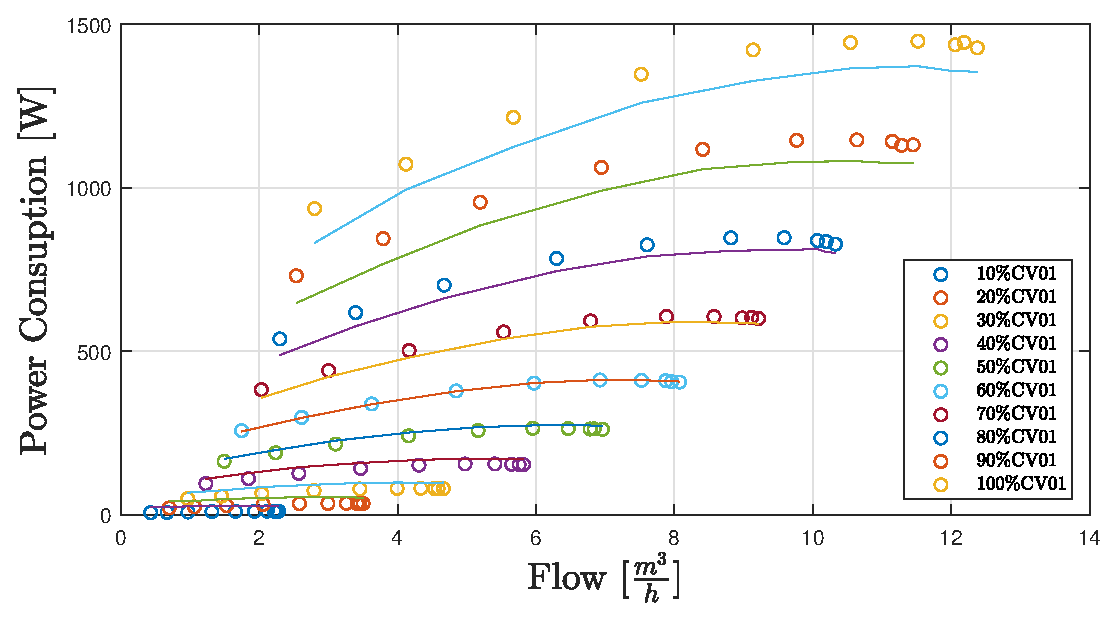
\includegraphics[width=0.8\textwidth]{figures/06ModelValidation/flowVsModeledPowerConsumption.eps}
	\caption{Flow Vs. Modeled Power Consumption}
	\label{fig:flowVsModeledPower}
\end{figure}
\begin{figure}[ht]
	\centering
	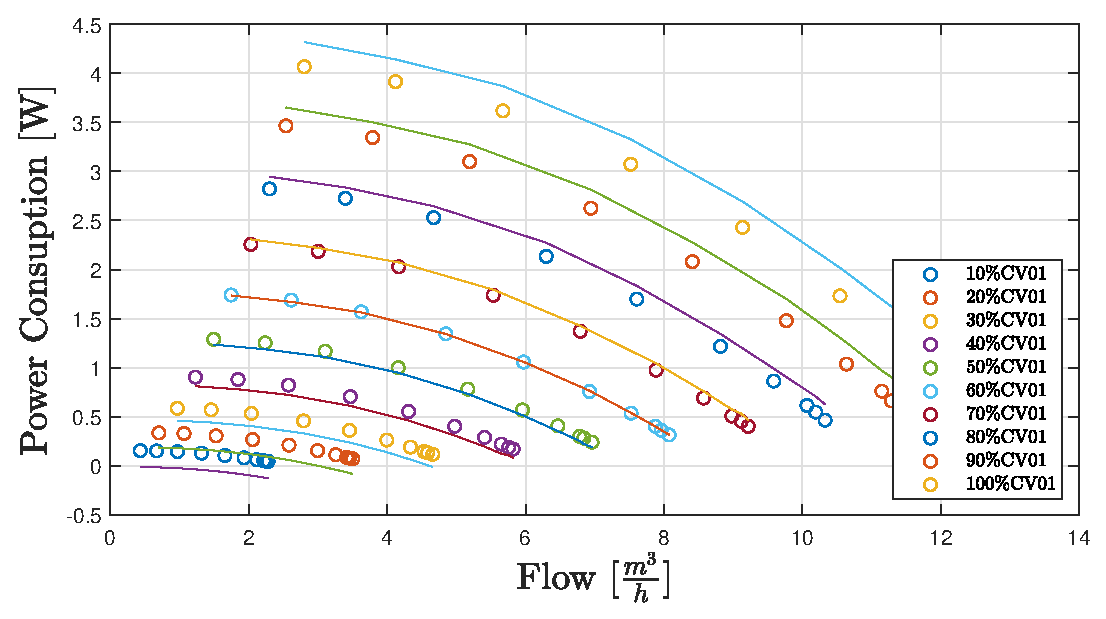
\includegraphics[width=0.8\textwidth]{figures/06ModelValidation/flowVsModeledPressure.eps}
	\caption{Flow Vs. Modeled Pressure}
	\label{fig:flowVsModeledPressure}
\end{figure}

As expected, the models are able to approximate the pump curves, that are closer to the actual pump speed 
the models were determined for. They are not as accurate overall as expected. 
The modelling errors could come as a result of many factors, however, there is room for improvement. 
As with the case of the pressure sensors, we were not able to determine accurate values for 
the pump speeds. Again, we have used gains and offsets provided to us. Additionally, as stated in \cite{Yang2010}
motor and drive efficiency are not accounted for.

\section{Dynamic Modelling}
We determined the coefficients for our P, I, and D using Ziegler Nichols tuning method.
The results both in theory and practice can be seen below. Figure \ref{fig:modeledPI2} represents the model for the PI -
Controller, while Figure \ref{fig:actualPI2} represents the output of the system using the same controller.

\begin{figure}[H]
	\centering
	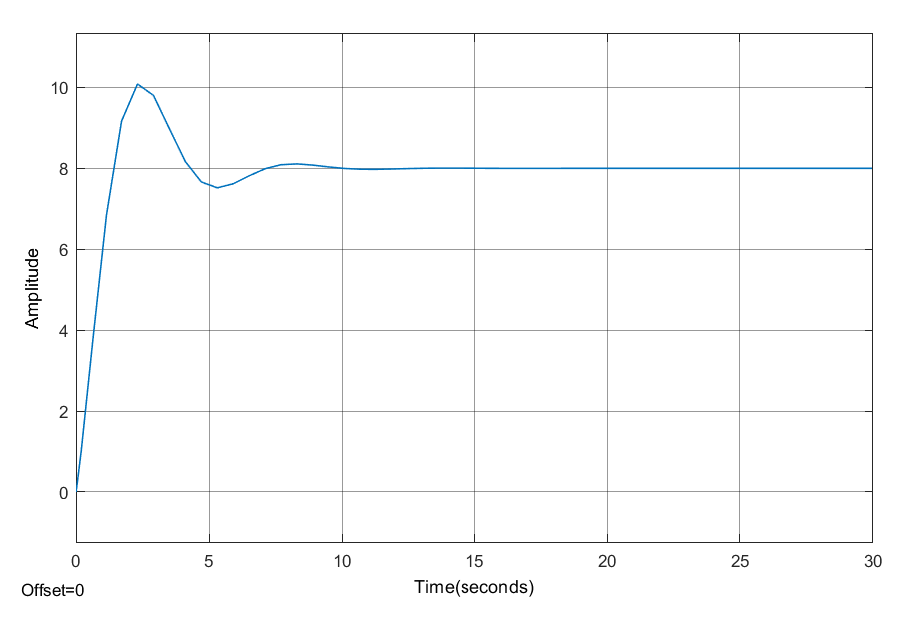
\includegraphics[width=0.7\textwidth]{figures/06ModelValidation/modelPI.eps}
	\caption{Modeled PI Controller}
	\label{fig:modeledPI2}
\end{figure}
\vspace{-5mm}
\begin{figure}[H]
    \centering
    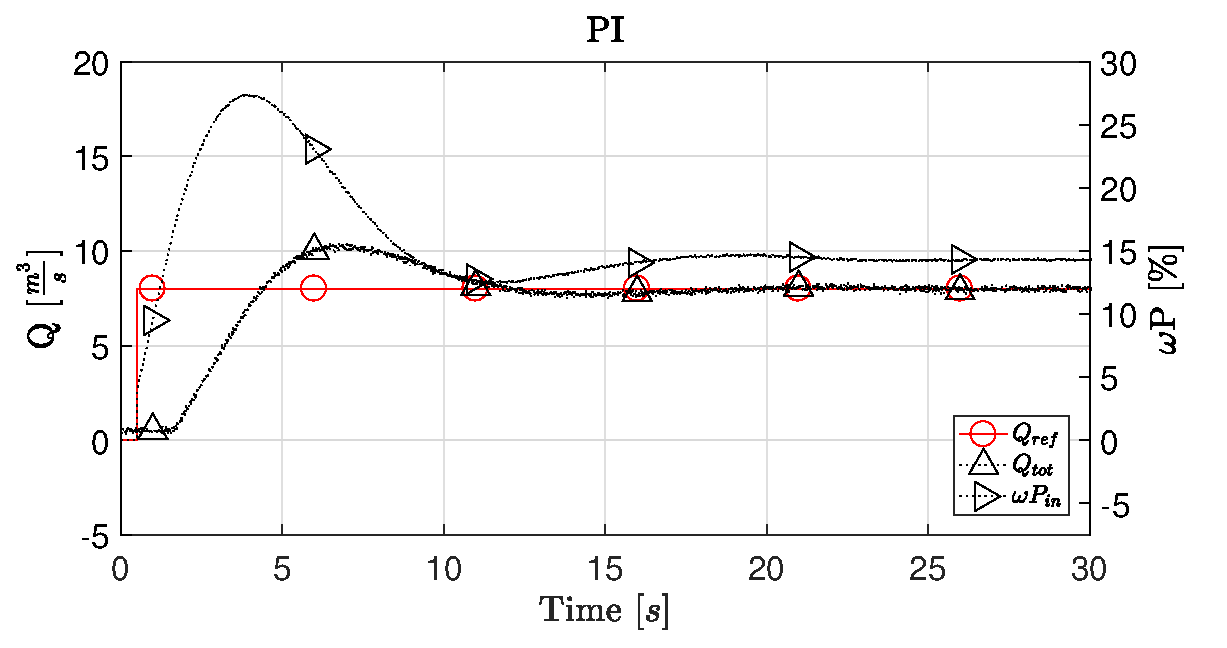
\includegraphics[width=\textwidth]{figures/07controllerDesign/PItest.eps}
    \caption{Actual PI Controller}
	\label{fig:actualPI2}
\end{figure}
The output of the model is quite similar to the output of the setup, with the exception of the delayed step input.
Additionally, the model seems to converge faster to the setpoint.

The model for the PID - Controller also presents strong similarities with the actual output of the setup.
The comparison can be seen in figures \ref{fig:modeledPID2} and \ref{fig:actualPID2}.
\begin{figure}[H]
	\centering
	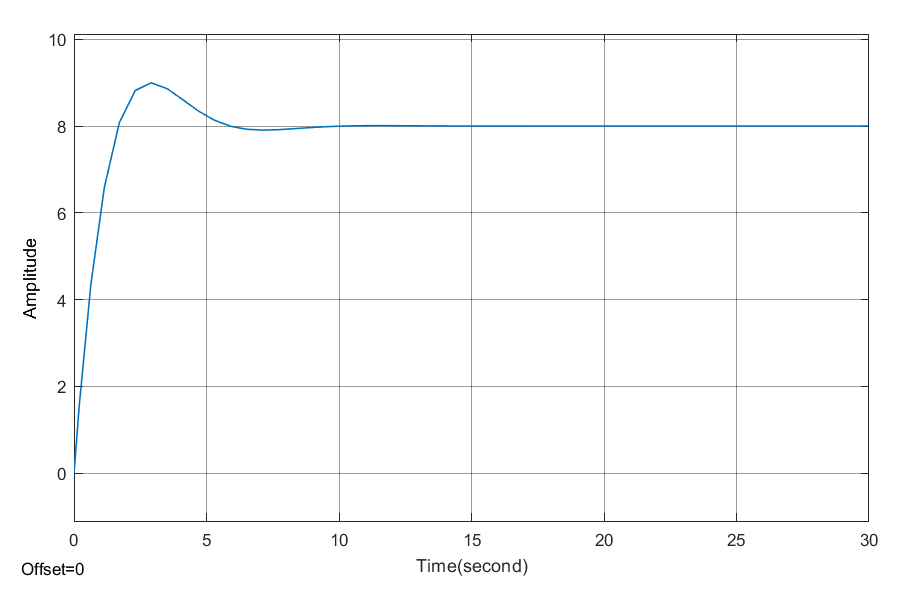
\includegraphics[width=0.7\textwidth]{figures/06ModelValidation/modelPID.eps}
	\caption{Modeled PID Controller}
	\label{fig:modeledPID2}
\end{figure}
\vspace{-5mm}
\begin{figure}[H]
    \centering
    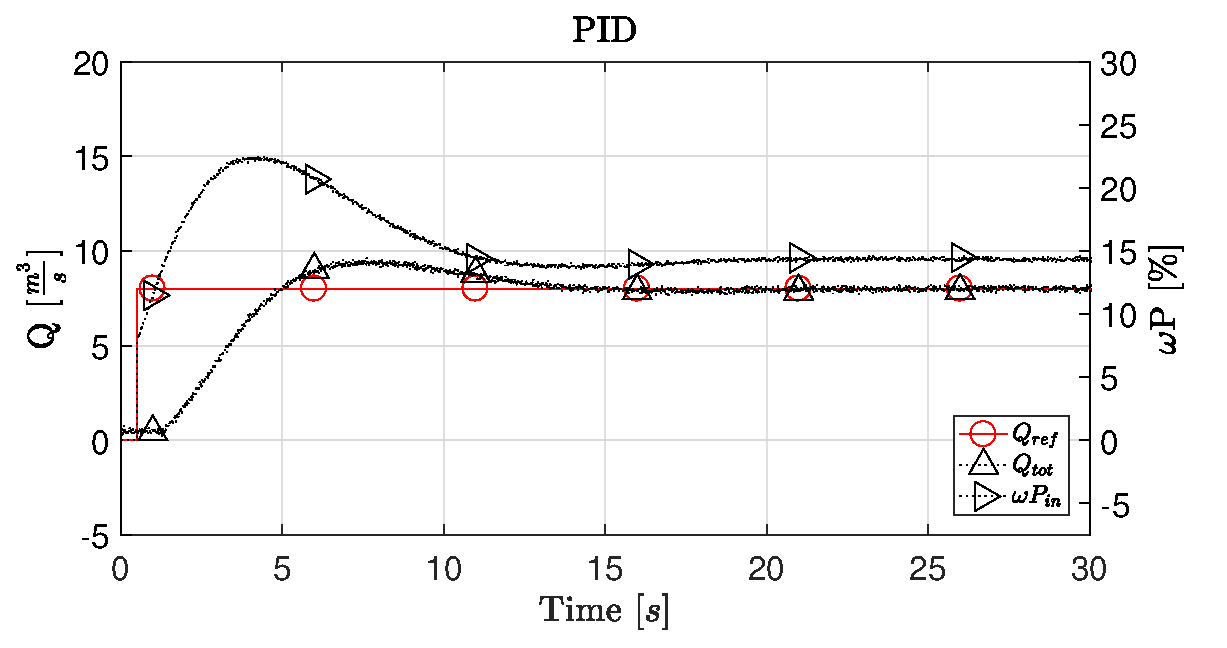
\includegraphics[width=\textwidth]{figures/07controllerDesign/PIDtest.eps}
    \caption{Actual PID Controller}
	\label{fig:actualPID2}
\end{figure}
Same can be noticed for the PID - Controller, the step input for the physical setup is given 0.5 seconds later.
The model also converges faster to the setpoint. This might be due to dynamic properties of the flow, which might 
not be properly modeled using the transfer function.